\let\negmedspace\undefined
\let\negthickspace\undefined
\documentclass[journal]{IEEEtran}
\usepackage[a5paper, margin=10mm, onecolumn]{geometry}
%\usepackage{lmodern} % Ensure lmodern is loaded for pdflatex
\usepackage{tfrupee} % Include tfrupee package

\setlength{\headheight}{1cm} % Set the height of the header box
\setlength{\headsep}{0mm}     % Set the distance between the header box and the top of the text

\usepackage{gvv-book}
\usepackage{gvv}
\usepackage{cite}
\usepackage{amsmath,amssymb,amsfonts,amsthm}
\usepackage{algorithmic}
\usepackage{graphicx}
\usepackage{textcomp}
\usepackage{xcolor}
\usepackage{txfonts}
\usepackage{listings}
\usepackage{enumitem}
\usepackage{mathtools}
\usepackage{gensymb}
\usepackage{comment}
\usepackage[breaklinks=true]{hyperref}
\usepackage{tkz-euclide} 
\usepackage{listings}
% \usepackage{gvv}                                        
\def\inputGnumericTable{}                                 
\usepackage[latin1]{inputenc}                                
\usepackage{color}                                            
\usepackage{array}                                            
\usepackage{longtable}                                       
\usepackage{calc}                                             
\usepackage{multirow}                                         
\usepackage{hhline}                                           
\usepackage{ifthen}                                           
\usepackage{lscape}
\begin{document}
\bibliographystyle{IEEEtran}
\title{10.2.8}
\author{EE25BTECH11002 - Achat Parth Kalpesh }
{\let\newpage\relax\maketitle}
\renewcommand{\thefigure}{\theenumi}
\renewcommand{\thetable}{\theenumi}
\setlength{\intextsep}{10pt} % Space between text and floats
\numberwithin{equation}{enumi}
\numberwithin{figure}{enumi}
\renewcommand{\thetable}{\theenumi}
\parindent 0px



\textbf{Question:}\\
The shortest distance from the point (2,7) to the circle $x^2+y^2- 14x-10y-151=0$ is equal to 5 \\
\textbf{Solution:}\\
The general equation of a circle is
\begin{align}
\label{1}
\vec{x}^T\vec{x} + 2\vec{u}^T\vec{x} + f = 0
\end{align}
where
\begin{align}
\vec{x} = \myvec{x \\ y},  \quad \vec{u} = \myvec{-7 \\ -5}, \quad f = -151
\end{align}

The center and radius are given by
\begin{align}
\vec{C} &= -\vec{u} = \myvec{7 \\ 5} \\
r &= \sqrt{\vec{u}^T\vec{u} - f}\\
r &= 15
\end{align}
Let the given point be $\vec{P}$
\begin{align}
\label{6}
\vec{P} = \myvec{2 \\ 7}
\end{align}
The distance between $\vec{P}$ and $\vec{C}$ is
\begin{align}
\norm{\vec{P} - \vec{C}} &= \sqrt{(\vec{P} - \vec{C})^T(\vec{P} - \vec{C})} \\
&= \sqrt{(2-7)^2 + (7-5)^2} \\
&= \sqrt{25 + 4} = \sqrt{29}
\end{align}

Substituting \eqref{6} in \eqref{1}\\
\begin{align}
    \vec{P}^T\vec{P} + 2\vec{u}^T\vec{P} + f < 0
\end{align}

The shortest distance of the point inside the circle is given as
\begin{align}
d = r - \norm{\vec{P} - \vec{C}}
\end{align}
Hence,
\begin{align}
d &= 15 - \sqrt{29}
\end{align}
Thus the shortest distance from the point (2,7) to the circle $x^2+y^2- 14x-10y-151=0$ is not equal to 5, it's 15 - $\sqrt{29}$

\begin{figure}[h!]
    \centering
    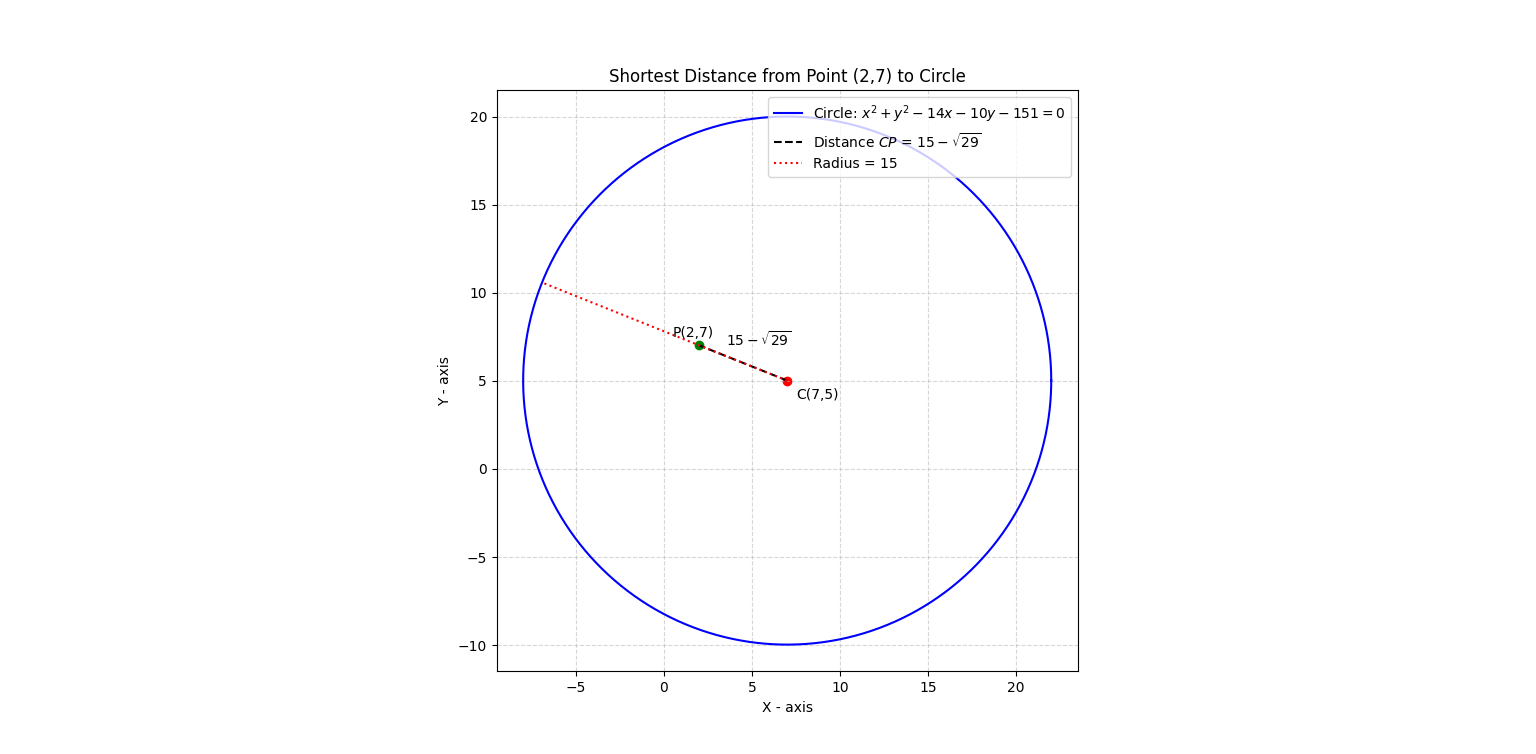
\includegraphics[width=\columnwidth]{figs/figure_py.png}
    \caption{Shortest Distance from Point (2,7) to Circle}
    \label{fig:fig}
 \end{figure}
\end{document}